\section{Theory}

The dielectric constant, also known as the relative permittivity, plays a vital role in understanding how a material responds to an applied electric field. This property is crucial in the design and optimisation of electronic devices, capacitors, and insulating materials, making it an essential parameter in modern technology.

Electrostatic processes in vacuum can be described by Maxwell’s equations as,

\begin{align}
    \oiint \vect{E} \cdot \vect{dA} &= \frac{Q}{\varepsilon_o}\\
    \oint \vect{E} \cdot \vect{dr} &= 0
\end{align}

where $\vect{E}$ is the electric field intensity, $Q$ is the charge enclosed by surface $A$ and $\varepsilon_o$ is the permittivity of free space. For a capacitor with two parallel plates of surface area $A$, if a potential difference $U_c$ is applied, an electric field $\vect{E}$ is formed between them, given by,

\begin{align}
    U_c = \int_1^2 \vect{E} \cdot \vect{dr}
\end{align}

\begin{figure}[H]
    \centering
    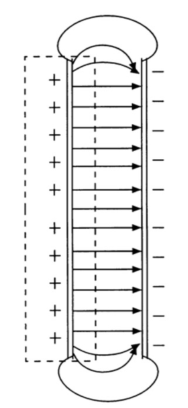
\includegraphics[height=0.8\columnwidth]{images/f1.png}
    \caption{Electric field lines between the capacitor plates}
    \label{fig:1}
\end{figure}

Due to this electric field, an equal amount of positive and negative charge is formed on both of the capacitor plates respectively. Assuming field lines between the plates to be perpendicular to the surface, using Eqn. (1) and (3), 

\begin{align}
    \frac{Q}{\varepsilon_o} = \frac{U_c}{d}A
\end{align}

for small distances $d$.
Since the charge on a capacitor is directly proportional to the potential difference between the plates, one can write,

\begin{align}
    Q = CU_c = \varepsilon_o\frac{U_cA}{d}
\end{align}

where $C$ --- the constant of proportionality --- is the capacitance of the capacitor. From Eq (5), we can infer that,

\begin{align}
    C = \frac{\varepsilon_oA}{d}
\end{align}

which shows that the capacitance is inversely proportional to the distance between the plates and directly proportional to the area of the plates. These are the intrinsic properties of a particular capacitor.

\subsection*{Dielectric between the Capacitor Plates}

Eq. (6) is derived with the assumption that there is vaccum between the plates, which has to be modified with the introduction of a dielectric (insulating material) between the plates. 

Dielectrics have no free moving charge carriers, as metals have, but they do have positive nuclei and negative electrons, which can arrange itself along the lines of an applied electric field $\vect{E_0}$. Formerly non-polar molecules thus get polarized and behave as locally stationary dipoles. The effects of the single dipoles cancel each other macroscopically inside the dielectric, but not on the surface. Hence the surfaces will possess a stationary charge, called a free charge. The free  charges in turn weaken the effective electric field $\vect{E}$ as given below,

\begin{align}
    \vect{E} =\frac{\vect{E_0}}{\varepsilon_r}
\end{align}

where $\varepsilon_r$ is the relative permittivity (or dielectric constant) of the medium. 

\begin{figure}[H]
    \centering
    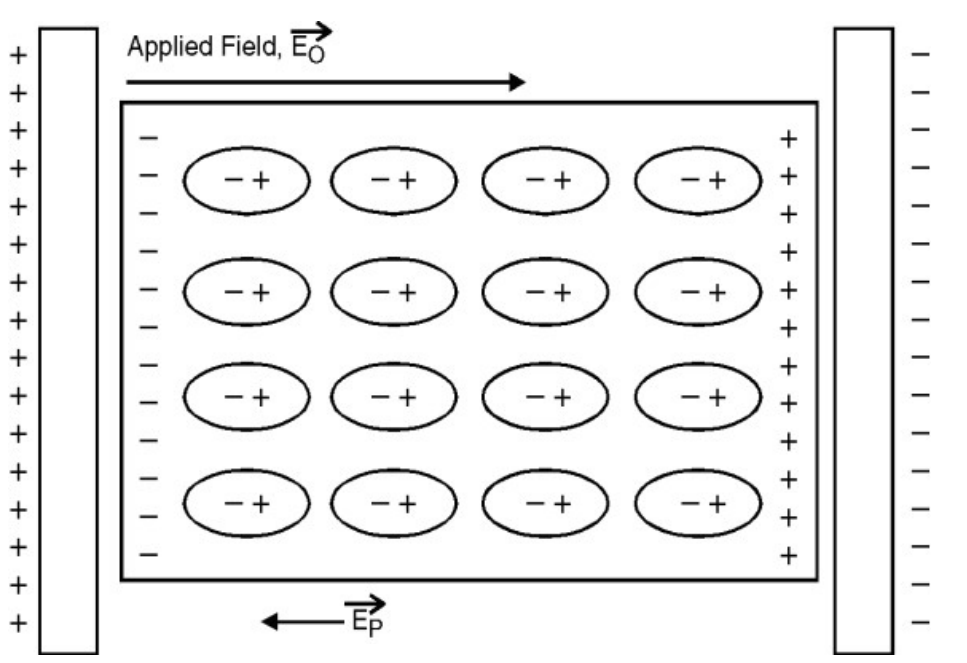
\includegraphics[width=0.8\columnwidth]{images/f3.png}
    \caption{Electric field lines between capacitor plates with a dielectric in between. Notice the dipoles aligned in the directtion of the external electric field.}
    \label{fig:2}
\end{figure}

The induced electric field $\vect{E_P}$ due to these charges will be in opposite direction to the applied electric field. If $\vect{P}$ is the polarization vector of the medium,

\begin{align}
    \vect{E_P} &= \vect{E_0} - \vect{E} = \vect{E_0} \left(1 - \frac{1}{\varepsilon_r}\right) \nonumber\\
    &= \frac{\vect{P}}{\varepsilon_o}
\end{align}

The electric displacement vector for an isotropic medium is defined as,

\begin{align}
    \vect{D} = \varepsilon \vect{E} = \varepsilon_o \varepsilon_r \vect{E} = \varepsilon_o \vect{E} + \vect{P}
\end{align}

where $\varepsilon$ is the electrical permittivity of the dielectric medium. When a dielectric is inserted between the capacitor plates, according to Eq. (3), voltage $U_c$ between the plates is reduced by the dielectric constant, $\varepsilon_r$, as compared to voltage in vacuum. Since the charge stored is constant, the capacitance will increase by a factor of $\varepsilon_r$.

\begin{align}
    C_\text{dielectric} = \varepsilon_r \varepsilon_o \frac{A}{d}\\
    \implies Q = \varepsilon_r \varepsilon_o \frac{AU_c}{d} 
\end{align}

Thus if one knows all the parameters, they can determine the dielectric constant of the medium by rearranging the above equation,

\begin{align}
    \varepsilon_r = \frac{d}{\varepsilon_oA} \cdot \frac{Q}{U_c}
\end{align}

\section{Experimental Setup}
The schematic for the setup is given in Fig (3). Initially the plate capacitors are charged using a high voltage supply. Then the charge is transferred to a known capacitor $C_\text{ref}$ (220nF). The voltage across $C_\text{ref}$, $V_o$ is measured by the voltmeter. From this, the total stored on the capacitor is calculated by $Q=V_oC_\text{ref}$. Subsequently, using Eq. (12), we can find the value of $\varepsilon_r$ for different media.

\begin{figure}[H]
    \centering
    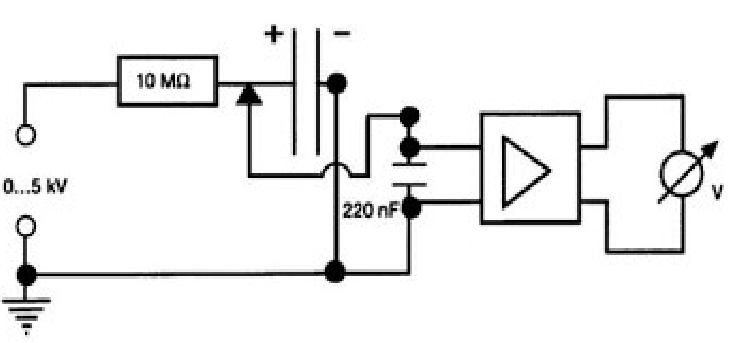
\includegraphics[width=0.95\columnwidth]{images/f2.png}
    \caption{Experimental setup schematic}
    \label{fig:3}
\end{figure}

\subsection*{Apparatus}

\begin{enumerate}
    \item Set of parallel plate capacitors (Diameter = 26 cm)
    \item High voltage power supply (0-10 kV)
    \item A 10 M$\Omega$ resistor
    \item Reference capacitor (220nF)
    \item Universal measuring amplifier
    \item Voltmeter
    \item Dielectric materials (Plastic and glass plates)
    \item Connecting cables, adapters, T-connectors
\end{enumerate}

